\documentclass[12pt]{article}

\usepackage{sbc-template}
\usepackage{graphicx,url}
\usepackage[utf8]{inputenc}
\usepackage[brazil]{babel}
\usepackage{amsmath}
\usepackage{subfig}
\usepackage{tikz}
\usetikzlibrary{positioning, arrows.meta, fit}

\sloppy

\title{ARIA: Pipeline Hierárquico \textit{Teacher-Student} para a\\
  Detecção Automatizada de Anomalias em Rochas Ornamentais}

\author{Henrique Machado de Oliveira\inst{1}\\
  \small Orientador: Everson Scherrer Borges\inst{1}}

\address{Instituto Federal do Espírito Santo (IFES) --- Campus Cachoeiro de
  Itapemirim\\
  Espírito Santo --- Brasil
  \email{rikemachado999@gmail.com}
}

\begin{document}

\maketitle

\begin{abstract}
  Surface quality control of ornamental stone slabs is still largely manual, making it subjective, prone to fatigue and hard to standardize. This work proposes ARIA, a hierarchical computer-vision pipeline in which a prior taxonomic classification (Xception) restricts the visual domain of a \textit{Teacher-Student} segmenter: the Segment Anything Model (SAM) generates calibrated annotations (pseudo-labels) that train specialist YOLO11-seg models. We hypothesize that domain-restricted specialist models reduce false positives compared to monolithic generalist ones. Initial results, obtained on the \textit{ice leke} lithotype, confirm that the foundation model segments relevant anomalies in a zero-shot setting when guided by lithology-calibrated prompts.

  \vspace{0.3cm}\noindent\normalfont\textbf{Keywords:} computer vision; ornamental stones; anomaly segmentation; foundation models; teacher-student learning.
\end{abstract}

\begin{resumo}
  O controle de qualidade superficial de chapas de rochas ornamentais ainda é majoritariamente manual, o que o torna subjetivo, sujeito à fadiga e de difícil padronização. Este trabalho propõe o ARIA (Análise e Reconhecimento Inteligente de Anomalias), um \textit{pipeline} hierárquico de visão computacional no qual uma classificação taxonômica prévia (Xception) restringe o domínio visual de um segmentador \textit{Teacher-Student}: o \textit{Segment Anything Model} (SAM) gera anotações calibradas (\textit{pseudo-labels}) que treinam modelos especialistas YOLO11-seg. A hipótese é que modelos especialistas, com domínio restrito, reduzem falsos positivos frente a modelos generalistas monolíticos. Os resultados iniciais, obtidos na litologia \textit{ice leke}, confirmam que o modelo de fundação segmenta anomalias relevantes em regime \textit{zero-shot} quando guiado por \textit{prompts} calibrados por litologia.

  \vspace{0.3cm}\noindent\normalfont\textbf{Palavras-chave:} visão computacional; rochas ornamentais; segmentação de anomalias; modelos de fundação; aprendizado \textit{Teacher-Student}.
\end{resumo}

\section{Introdução}

O controle de qualidade de chapas é uma etapa crítica da indústria de rochas ornamentais, setor estratégico para as exportações brasileiras e fortemente concentrado no Espírito Santo, principal polo produtor e exportador do país~\cite{stone_economy_bahiense2023}. A inspeção de anomalias superficiais --- fissuras, veios, manchas e oxidações --- é realizada de forma majoritariamente manual, dependendo da acuidade visual do operador~\cite{stone_inspection_vidal2013}. Esse processo é inerentemente subjetivo, suscetível à fadiga e de difícil padronização, com impacto direto na precificação e nas perdas industriais~\cite{stone_subjectivity_castro2018}.

A automação dessa inspeção por meio de visão computacional esbarra em dois obstáculos. O primeiro é a alta variabilidade geológica das rochas: uma feição que constitui anomalia comercial em uma litologia (uma fissura em mármore branco) pode ser um padrão natural esperado em outra (um veio mineral em granito). Modelos generalistas monolíticos, treinados sobre todas as litologias ao mesmo tempo, tendem a confundir essas feições e a gerar falsos positivos. O segundo é o custo da anotação: a rotulagem manual de milhares de imagens com defeitos sutis é onerosa e limitante para a adoção industrial.

Este trabalho propõe o ARIA (Análise e Reconhecimento Inteligente de Anomalias), um \textit{pipeline} hierárquico de Inteligência Artificial concebido para ser o núcleo inteligente da plataforma industrial Hartheus, voltada ao controle de qualidade de chapas. A proposta articula três estágios: um classificador taxonômico baseado na arquitetura Xception --- o DeepStoneAI, rede convolucional previamente desenvolvida e publicada pelo grupo~\cite{deepstoneai_moreira2025} ---, que identifica o domínio litológico da chapa; o \textit{Segment Anything Model} (SAM)~\cite{sam_kirillov2023}, que atua como Professor em uma arquitetura \textit{Teacher-Student}, gerando anotações automatizadas (\textit{pseudo-labeling}); e modelos YOLO11~\cite{yolo11_khanam2024}, que atuam como Alunos especialistas, otimizados para inferência rápida na linha de produção.

A pergunta de pesquisa que orienta o trabalho é: \textit{uma abordagem hierárquica --- na qual a classificação taxonômica prévia restringe o domínio visual do segmentador --- reduz os falsos positivos na detecção de anomalias superficiais em rochas ornamentais, em comparação a modelos generalistas monolíticos?} A hipótese central (H1) é que modelos especialistas hierárquicos, por conhecerem a aparência normal de cada litologia, apresentam menor índice de falsos positivos do que um modelo generalista único.

O objetivo geral é desenvolver e validar o \textit{pipeline} ARIA. Como objetivos específicos: (i) implementar o classificador taxonômico e integrá-lo ao roteamento do \textit{pipeline}; (ii) calibrar o SAM, por injeção de conhecimento de domínio, para gerar anotações por litologia; (iii) treinar modelos YOLO11 especialistas com as anotações do Professor; e (iv) comparar a abordagem hierárquica a um \textit{baseline} generalista em mAP e IoU, complementando a análise com validação qualitativa por especialistas do setor.

O restante do artigo está organizado da seguinte forma. A Seção~\ref{sec:fundamentacao} apresenta a fundamentação teórica; a Seção~\ref{sec:relacionados}, os trabalhos relacionados; a Seção~\ref{sec:metodologia} detalha a metodologia e o protocolo experimental; a Seção~\ref{sec:resultados} reporta os resultados iniciais; e a Seção~\ref{sec:conclusao} traz as considerações parciais e os trabalhos futuros.

\section{Fundamentação Teórica}
\label{sec:fundamentacao}

\subsection{Visão Computacional e Classificação Taxonômica}

A visão computacional moderna apoia-se em Redes Neurais Convolucionais (\textit{Convolutional Neural Networks} --- CNN), que extraem informações de imagens por meio de filtros que evidenciam texturas e formas~\cite{deeplearning_lecun2015}. Em um \textit{pipeline} hierárquico, a identificação do domínio de conhecimento --- a variedade litológica da rocha --- é a etapa primordial. Para essa tarefa, a arquitetura Xception~\cite{xception_chollet2017} apresenta alta eficiência por meio de convoluções separáveis em profundidade (\textit{depthwise separable convolutions}), reduzindo o custo computacional e mantendo elevada acurácia na etapa de roteamento do sistema.

\subsection{Segmentação de Imagens por Aprendizado Profundo}

A detecção de anomalias enquanto regiões delimitadas na imagem é, em essência, um problema de segmentação. Abordagens supervisionadas consolidadas incluem a U-Net~\cite{unet_ronneberger2015}, amplamente empregada em segmentação biomédica, e a Mask R-CNN~\cite{maskrcnn_he2017}, que estende a detecção de objetos com a predição de máscaras de instância; levantamentos recentes sistematizam a evolução dessas técnicas~\cite{segsurvey_minaee2021}. Tais métodos, contudo, exigem grandes volumes de dados anotados manualmente --- limitação crítica no domínio industrial de rochas, onde inexiste \textit{ground truth} padronizado. É justamente essa limitação que motiva o uso de um modelo de fundação como gerador de anotações, abordado a seguir.

\subsection{Modelos de Fundação e o \textit{Segment Anything Model}}

Nos últimos anos, a área avançou para o paradigma dos Modelos de Fundação (\textit{Foundation Models}) --- redes massivas treinadas em conjuntos de dados em larga escala, capazes de executar tarefas genéricas com alta precisão e sem treinamento específico (capacidade \textit{zero-shot}). Nesse contexto destaca-se o \textit{Segment Anything Model} (SAM)~\cite{sam_kirillov2023}, fundamentado na engenharia de \textit{prompts}: o modelo pode ser guiado por coordenadas, caixas delimitadoras ou texto para isolar objetos em uma imagem. A interpretação dos \textit{prompts} textuais apoia-se no CLIP~\cite{clip_radford2021}, que projeta texto e imagem em um espaço de \textit{embeddings} compartilhado, aproximando o vetor de uma palavra (como \textit{crack}) das regiões visualmente similares.

No domínio de rochas ornamentais, isso habilita a \textbf{injeção de conhecimento de domínio}: ao calibrar os \textit{prompts} e os limiares de confiança com as características visuais específicas de cada litologia, converte-se um modelo genérico em um segmentador especializado, evitando que feições geológicas naturais (veios) sejam confundidas com defeitos comerciais.

\subsection{Arquitetura \textit{Teacher-Student} e \textit{Pseudo-labeling}}

O principal gargalo para a adoção de visão computacional na indústria é a escassez de dados anotados manualmente (\textit{ground truth}). Para contornar essa limitação, a literatura emprega a transferência de conhecimento por meio da arquitetura \textit{Teacher-Student}~\cite{distill_hinton2015} acoplada à técnica de \textit{pseudo-labeling}~\cite{pseudolabel_lee2013}. Um modelo robusto e de alto custo computacional atua como Professor (neste trabalho, o SAM), processando imagens de forma \textit{offline} para gerar máscaras de segmentação. Essas anotações, denominadas \textit{pseudo-labels}, supervisionam o treinamento de um modelo Aluno, estatisticamente menor, porém otimizado para inferência rápida.

\subsection{Inferência em Tempo Real com YOLO}

No ambiente de manufatura contínua, em que prevalecem \textit{hardwares} com restrição de recursos (\textit{Edge Computing}), a velocidade de inferência é prioritária. O modelo Aluno adotado é a arquitetura YOLO (\textit{You Only Look Once})~\cite{yolo_redmon2016}, em sua versão 11~\cite{yolo11_khanam2024}, que processa extração de características (\textit{backbone}) e predição de máscaras (\textit{head}) em uma única passagem pela rede, atingindo altas taxas de quadros por segundo (FPS). Essa eficiência viabiliza a inferência em tempo real na linha de produção, requisito central da aplicação industrial proposta.

\subsection{Adoção Tecnológica e Indústria 4.0}

A inserção de um sistema de inspeção automatizada em chão de fábrica é, também, um problema de Sistemas de Informação. O Modelo de Aceitação de Tecnologia (\textit{Technology Acceptance Model} --- TAM)~\cite{tam_davis1989} indica que a utilidade percebida e a facilidade de uso são determinantes da adoção; a Teoria da Difusão de Inovações~\cite{diffusion_rogers2003} ressalta a necessidade de demonstrar vantagens relativas, como ganho de eficiência e padronização; e a Teoria Sociotécnica~\cite{sociotech_trist1951} lembra que o sucesso depende da harmonização entre os aspectos técnicos e os sociais do trabalho. Tais perspectivas situam o ARIA no contexto da Indústria 4.0~\cite{industry40_lee2014} --- a digitalização e a integração de IA aos processos produtivos --- e funcionam como referencial de apoio, não como objeto central de análise deste trabalho.

\section{Trabalhos Relacionados}
\label{sec:relacionados}

A inspeção visual automatizada (\textit{Automated Visual Inspection} --- AVI) para detecção de defeitos é tema consolidado em diversos setores industriais, com aplicações de IA em têxtil~\cite{avi_textile_sikka2024}, construção civil~\cite{avi_concrete_waqar2024}, alimentício~\cite{avi_food_chen2021} e soldagem aeronáutica~\cite{avi_welding_tsuzuki2022}. Levantamentos recentes sobre detecção de anomalias visuais industriais sistematizam essas abordagens e evidenciam um gargalo recorrente: a maioria depende de aprendizado supervisionado e, portanto, de grandes volumes de imagens anotadas manualmente~\cite{avi_anomaly_li2025}. Esse custo de anotação é particularmente limitante em domínios de alta variabilidade visual, como o de rochas ornamentais, em que cada litologia exige exemplos próprios.

No contexto específico das rochas ornamentais, os trabalhos existentes concentram-se na \textit{classificação} do tipo de rocha, e não na \textit{segmentação} de anomalias superficiais. Técnicas de aprendizado de máquina já foram aplicadas à classificação de pedras ornamentais~\cite{stone_lopez2010, stone_tereso2020}, e redes convolucionais profundas, à tipificação automatizada de rochas~\cite{rocktyping_baraboshkin2020}. No mesmo campus desta pesquisa, redes convolucionais já haviam sido exploradas para a classificação de chapas polidas~\cite{deepstone_araujo2022}; esse esforço evoluiu para o DeepStoneAI~\cite{deepstoneai_moreira2025}, classificador publicado pelo grupo e reaproveitado diretamente como estágio de classificação taxonômica do ARIA.

Identifica-se, assim, uma lacuna: a detecção de anomalias superficiais em rochas ornamentais permanece pouco explorada, enquanto as abordagens de AVI disponíveis esbarram no custo da anotação manual. O diferencial deste trabalho está em endereçar essa lacuna ao combinar a classificação litológica prévia, a segmentação por um modelo de fundação calibrado por litologia --- que dispensa anotação manual extensiva por meio de \textit{pseudo-labeling} --- e a destilação para um modelo de inferência rápida, adequado à linha de produção.

\section{Metodologia}
\label{sec:metodologia}

\subsection{Tipo de Pesquisa}

O trabalho classifica-se como pesquisa aplicada, de natureza experimental e abordagem mista (quantitativa e qualitativa). É aplicada por buscar resolver um problema prático do setor industrial capixaba; é experimental por manipular variáveis, arquiteturas e hiperparâmetros para observar seus efeitos nas métricas de acurácia, precisão e velocidade de inferência.

\subsection{Conjunto de Dados}

O conjunto de dados reúne aproximadamente 34.630 imagens industriais reais de chapas~\cite{dataset_araujo2023}, distribuídas em 45 litologias (tipos comerciais de rocha) e preservando o desbalanceamento natural da produção --- algumas variedades são muito mais frequentes que outras. A alta variabilidade, tanto entre litologias quanto dentro de uma mesma litologia (lote, iluminação, acabamento), é justamente o fator que motiva a abordagem especialista. As anomalias superficiais consideradas na calibração do SAM estão resumidas na Tabela~\ref{tab:anomalias}; vale notar que o mesmo padrão visual pode constituir defeito em uma litologia e característica estética em outra, o que reforça a necessidade de restringir o domínio antes de segmentar.

\begin{table}[ht]
\centering
\caption{Tipos de anomalia superficial considerados na calibração do SAM.}
\label{tab:anomalias}
\begin{tabular}{ll}
\hline
\textbf{Anomalia} & \textbf{Descrição} \\
\hline
\textit{crack} & Fissuras e trincas na superfície \\
\textit{vein} & Veios minerais; podem ser anomalia ou característica natural \\
\textit{stain} & Manchas e descolorações \\
\textit{dark patches} & Áreas escuras / oxidação em rochas claras \\
\textit{light spot} & Pontos claros em rochas escuras \\
\hline
\end{tabular}
\end{table}

\subsection{Procedimentos Metodológicos}

O desenvolvimento do ARIA será conduzido em etapas sequenciais, validando-se cada módulo antes da integração final:

\begin{enumerate}
  \item \textbf{Coleta e pré-processamento de dados:} constituição do banco de imagens industriais reais descrito acima, representando diferentes litologias e preservando o desbalanceamento natural de classes (anomalias sutis \textit{vs.} chapas íntegras).
  \item \textbf{Classificação taxonômica:} treinamento e validação da rede Xception (DeepStoneAI~\cite{deepstoneai_moreira2025}) para classificar o domínio litológico da chapa, estabelecendo a restrição de domínio para a etapa seguinte.
  \item \textbf{Calibração do Professor e geração de \textit{pseudo-labels}:} injeção de conhecimento de domínio no SAM. Um arquivo de configuração estruturado (\texttt{rock\_prompts.json}) define os \textit{prompts} e os limiares de confiança específicos de cada rocha, e o SAM processa o \textit{dataset} \textit{offline}, gerando as anotações. Nesta versão, todas as anomalias são tratadas como uma única classe genérica (rotulagem binária), pois a distinção semântica entre tipos de anomalia depende da qualidade dos \textit{embeddings} de texto, ainda não validada de forma independente; a rotulagem multiclasse fica registrada como extensão futura.
  \item \textbf{Treinamento do Aluno (YOLO11):} alimentação do motor de inferência com os \textit{pseudo-labels} da etapa anterior, maximizando a taxa de FPS e a assertividade na detecção.
  \item \textbf{Validação:} avaliação quantitativa por mAP e IoU, complementada pela validação qualitativa das anotações por especialistas do setor de rochas ornamentais.
\end{enumerate}

\subsection{Protocolo Experimental}

O experimento central avalia a hipótese da especialização hierárquica comparando dois \textit{pipelines} treinados sobre a mesma arquitetura YOLO11-seg. No \textit{pipeline} especialista (ARIA), o classificador Xception identifica o tipo litológico e seleciona os \textit{prompts} calibrados correspondentes, resultando em \textbf{45 modelos especializados} --- um por tipo de rocha, treinado exclusivamente nas anotações daquela litologia. No \textit{pipeline} \textit{baseline} (generalista), o estágio de classificação é ausente: o SAM usa uma configuração genérica de \textit{prompts} para todas as rochas e um \textbf{único modelo} YOLO é treinado com as anotações de todos os tipos. A comparação isola a variável da hierarquia --- a quantidade de modelos (45 \textit{vs.} 1) e a especificidade das anotações ---, permitindo medir o ganho da abordagem especialista.

\subsection{Protocolo de Avaliação}

A avaliação quantitativa apoia-se em duas métricas padrão de segmentação. A Interseção sobre União (\textit{Intersection over Union} --- IoU) mede a sobreposição entre a máscara predita $A$ e a máscara de referência $B$ (Equação~\ref{eq:iou})~\cite{iou_mahmood2021}. A precisão média (\textit{mean Average Precision} --- mAP) consolida o desempenho em $N$ classes como a média da precisão média ($\mathrm{AP}$) por classe (Equação~\ref{eq:map})~\cite{voc_everingham2010}.

\begin{equation}
  \mathrm{IoU} = \frac{|A \cap B|}{|A \cup B|}
  \label{eq:iou}
\end{equation}

\begin{equation}
  \mathrm{mAP} = \frac{1}{N} \sum_{i=1}^{N} \mathrm{AP}_i
  \label{eq:map}
\end{equation}

Como o \textit{ground truth} é gerado pelo próprio SAM, sem anotação humana paralela pixel a pixel, a comparação quantitativa entre Professor e Aluno é válida, mas deve ser contextualizada: mAP e IoU são sensíveis à qualidade da anotação. Por isso, a validação qualitativa por especialistas do setor --- que avaliam se as segmentações fazem sentido técnico-industrial --- complementa a análise. A subjetividade da anotação é tratada como parte da discussão metodológica, não como um problema a omitir.

\subsection{Ferramentas e Tecnologias}

O desenvolvimento utiliza Python com o \textit{framework} PyTorch~\cite{pytorch_paszke2019} para construção, treinamento e inferência dos modelos, e a plataforma CUDA (NVIDIA) para processamento paralelo em GPU. A Figura~\ref{fig:arquitetura} ilustra o fluxo hierárquico do ARIA, da classificação taxonômica à segmentação pelas arquiteturas \textit{Teacher-Student}.

\begin{figure}[ht]
  \centering
  \resizebox{\textwidth}{!}{%
  \begin{tikzpicture}[
    node distance=0.55cm and 0.7cm,
    box/.style={draw, rounded corners, align=center, minimum height=1.2cm,
      text width=2.8cm, font=\small, inner sep=4pt},
    io/.style={draw, align=center, font=\small, text width=2.0cm, inner sep=4pt},
    arr/.style={-{Latex[length=2.2mm]}, thick}
  ]
    \node[io] (in) {Imagem da chapa};
    \node[box, right=of in] (xc) {\textbf{Xception}\\classifica o tipo
      litológico};
    \node[box, right=of xc] (sam) {\textbf{SAM} (Professor)\\anotações
      calibradas por litologia};
    \node[box, right=of sam] (yolo) {\textbf{YOLO11-seg} (Aluno)
      $\times\,45$\\inferência rápida};
    \node[io, right=of yolo] (out) {Polígonos de anomalias};
    \draw[arr] (in) -- (xc);
    \draw[arr] (xc) -- (sam);
    \draw[arr] (sam) -- (yolo);
    \draw[arr] (yolo) -- (out);
    \node[draw, dashed, fit=(sam)(yolo), inner sep=9pt,
      label={[font=\small\itshape]above:Teacher--Student}] {};
  \end{tikzpicture}%
  }
  \caption{\textit{Pipeline} hierárquico do ARIA: a classificação taxonômica
    (Xception) restringe o domínio visual do segmentador especialista
    \textit{Teacher-Student} (SAM gera as anotações que treinam os modelos
    YOLO11). Fonte: elaborado pelo autor.}
  \label{fig:arquitetura}
\end{figure}

\section{Resultados Iniciais}
\label{sec:resultados}

Esta seção apresenta as primeiras evidências práticas do desenvolvimento, em consonância com a metodologia. Reportam-se o estado validado do estágio de classificação e os resultados em andamento do segmentador especialista.

\subsection{Classificação Litológica (DeepStoneAI)}

O estágio de classificação taxonômica do ARIA reaproveita o DeepStoneAI, avaliado em trabalho anterior do grupo sobre as 45 litologias do conjunto de dados~\cite{deepstoneai_moreira2025}. Entre quatro arquiteturas comparadas, a Xception obteve a maior acurácia (Tabela~\ref{tab:deepstone}), com a maior parte dos tipos de rocha perfeitamente classificada e confusão mínima apenas entre variedades visualmente semelhantes. Esse desempenho valida o primeiro estágio do \textit{pipeline} e sustenta um roteamento confiável das chapas para os segmentadores especialistas correspondentes.

\begin{table}[ht]
\centering
\caption{Acurácia de classificação reportada pelo DeepStoneAI, por arquitetura~\cite{deepstoneai_moreira2025}.}
\label{tab:deepstone}
\begin{tabular}{lc}
\hline
\textbf{Arquitetura} & \textbf{Acurácia} \\
\hline
Xception & 99,21\% \\
Inception-ResNetV2 & 97,94\% \\
MobileNetV2 & 91,26\% \\
EfficientNetV2-L & 54,04\% \\
\hline
\end{tabular}
\end{table}

\subsection{Geração de Anotações pelo Professor (SAM)}

O foco atual do desenvolvimento está na etapa do segmentador especialista, mais especificamente na atuação do SAM como Professor. Os resultados a seguir foram obtidos na rocha \textit{ice leke}, primeiro litótipo a ter seus \textit{prompts} e limiares de confiança calibrados e validados no arquivo \texttt{rock\_prompts.json}. A partir de uma imagem industrial real da chapa, o SAM foi guiado por \textit{prompts} de linguagem natural calibrados para a litologia (injeção de conhecimento de domínio), segmentando as anomalias superficiais sem qualquer treinamento prévio específico para rochas ornamentais (capacidade \textit{zero-shot}). A Figura~\ref{fig:resultado_combined} contrapõe a imagem original às máscaras de segmentação sobrepostas, geradas de forma totalmente automatizada.

\begin{figure}[ht]
  \centering
  \subfloat[Imagem original da chapa\label{subfig:original}]{%
    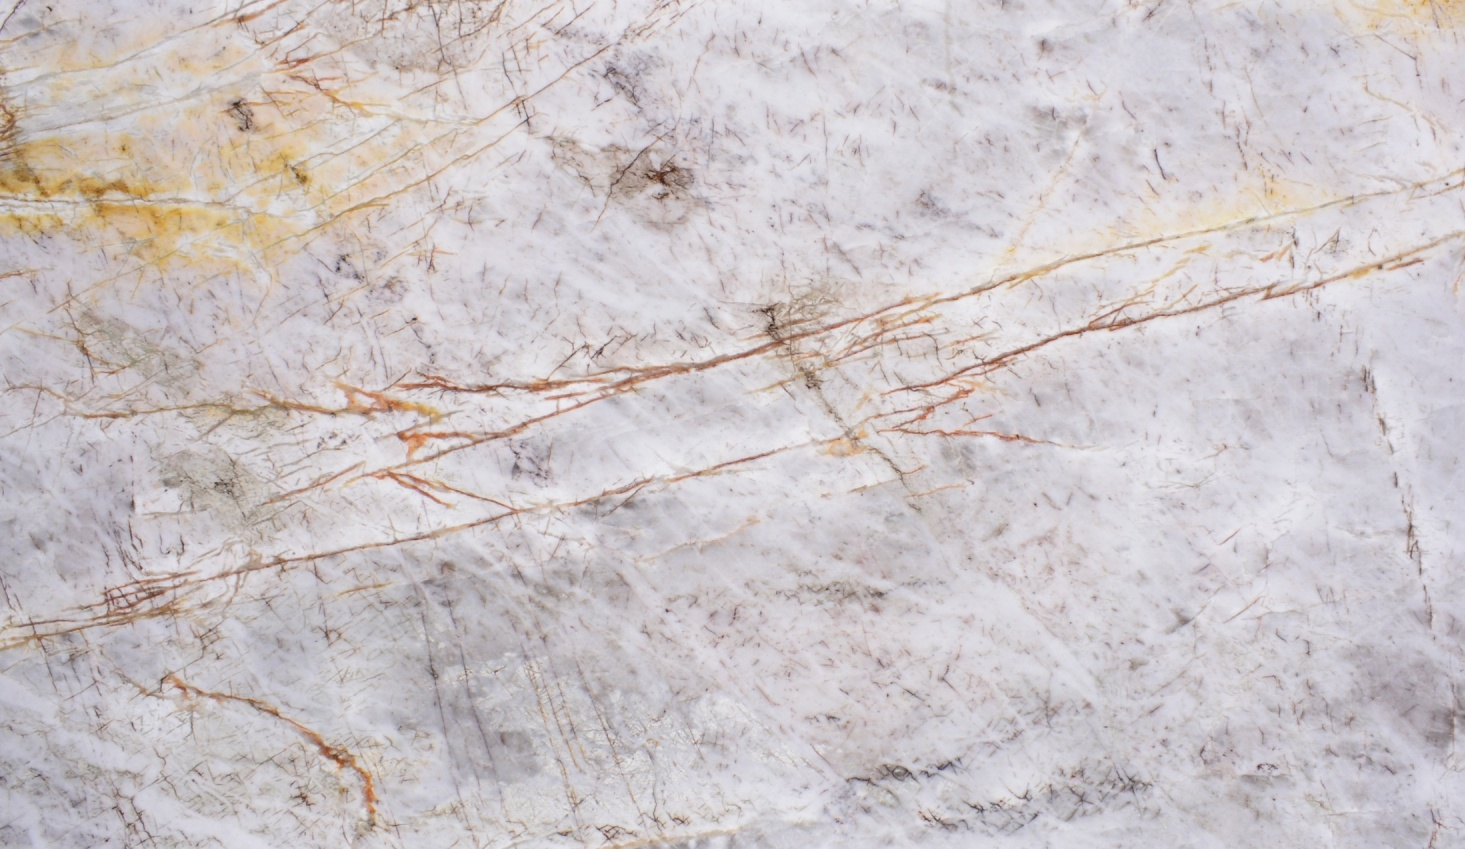
\includegraphics[width=0.45\textwidth]{figuras/sample_ice_leke_original.jpg}}
  \hfill
  \subfloat[Anotações geradas pelo SAM\label{subfig:combined}]{%
    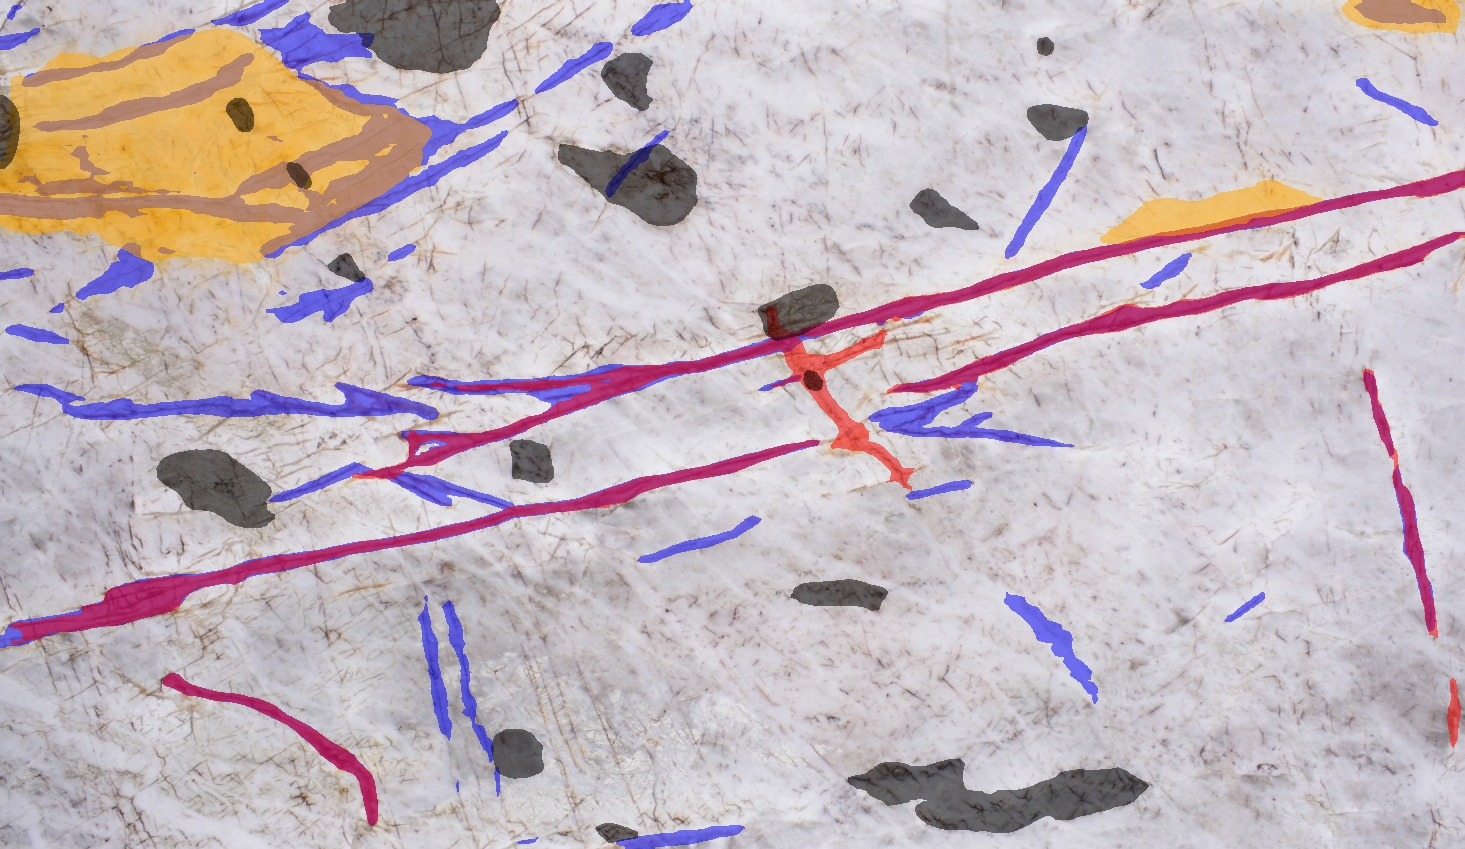
\includegraphics[width=0.45\textwidth]{figuras/sample_ice_leke_combined.jpg}}
  \caption{Segmentação automatizada de anomalias gerada pelo SAM na rocha
    \textit{ice leke}: imagem original (a) e máscaras de anomalias sobrepostas
    (b). Fonte: elaborado pelo autor.}
  \label{fig:resultado_combined}
\end{figure}

\subsection{Decomposição por Tipo de Anomalia}

Cada \textit{prompt} calibrado atua sobre um tipo específico de irregularidade. A Figura~\ref{fig:resultado_decomposto} apresenta as máscaras isoladas por categoria --- fissuras (\textit{crack}), veios minerais (\textit{vein}), manchas (\textit{Stain}) e áreas escuras (\textit{Dark patches}) ---, evidenciando a capacidade do modelo de distinguir diferentes feições visuais a partir de descrições textuais.

\begin{figure}[ht]
  \centering
  \subfloat[\textit{crack} (fissuras)\label{subfig:crack}]{%
    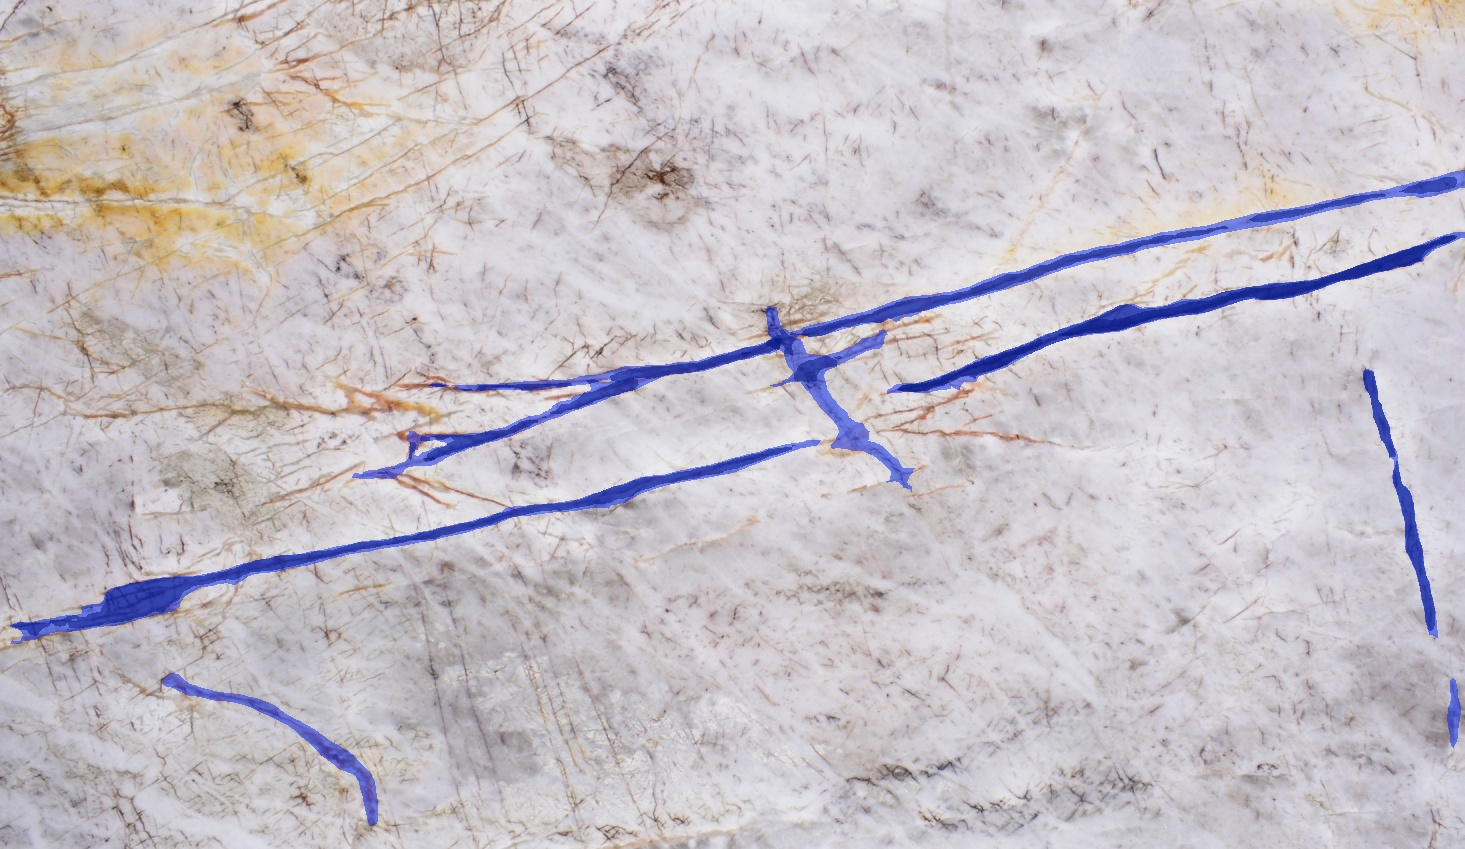
\includegraphics[width=0.45\textwidth]{figuras/sample_ice_leke_crack.jpg}}
  \hfill
  \subfloat[\textit{vein} (veios)\label{subfig:vein}]{%
    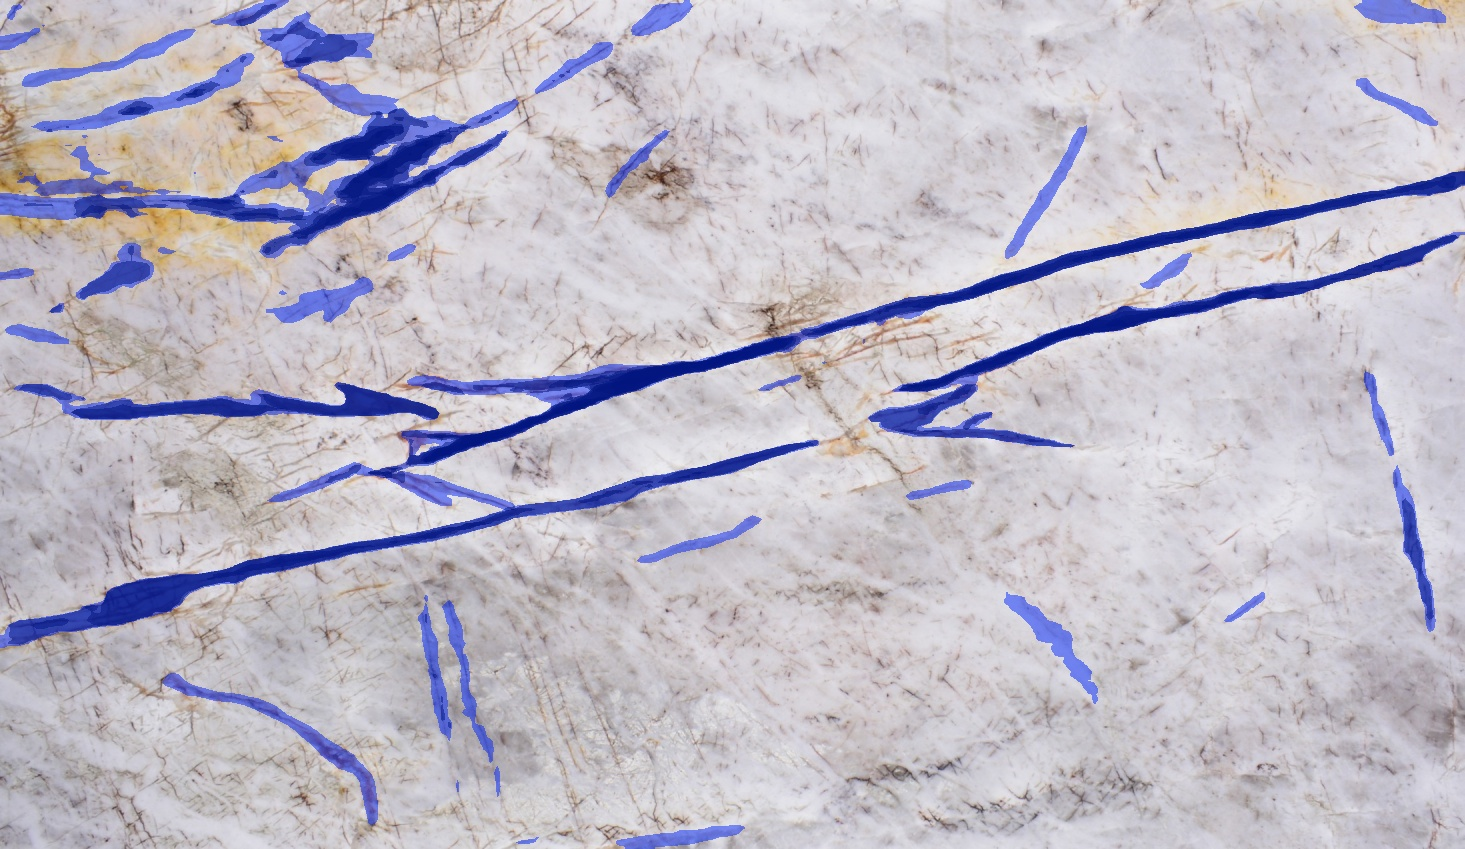
\includegraphics[width=0.45\textwidth]{figuras/sample_ice_leke_vein.jpg}}
  \\[0.4cm]
  \subfloat[\textit{Stain} (manchas)\label{subfig:stain}]{%
    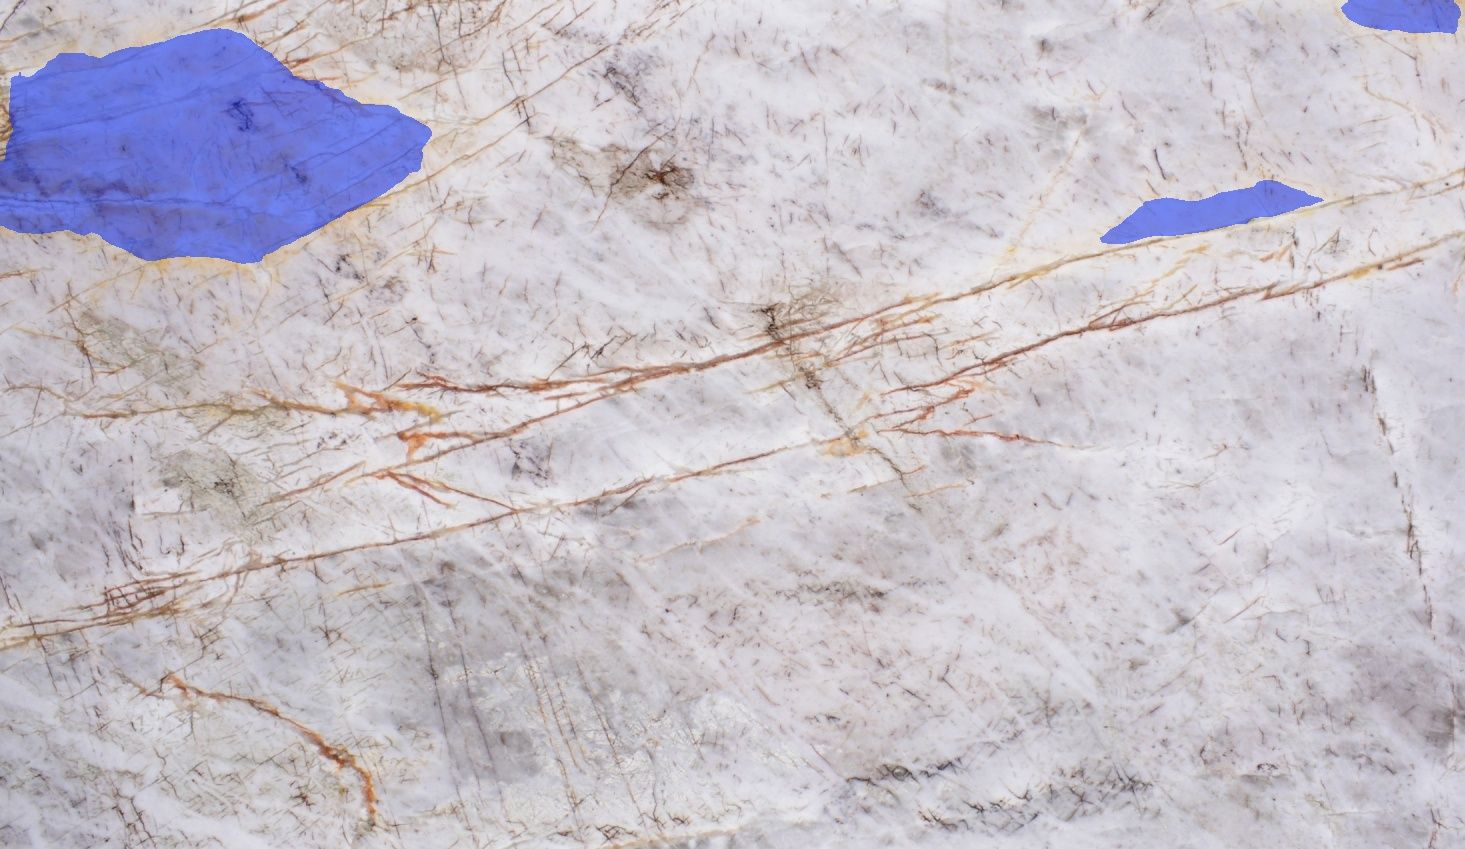
\includegraphics[width=0.45\textwidth]{figuras/sample_ice_leke_stain.jpg}}
  \hfill
  \subfloat[\textit{Dark patches} (áreas escuras)\label{subfig:darkpatches}]{%
    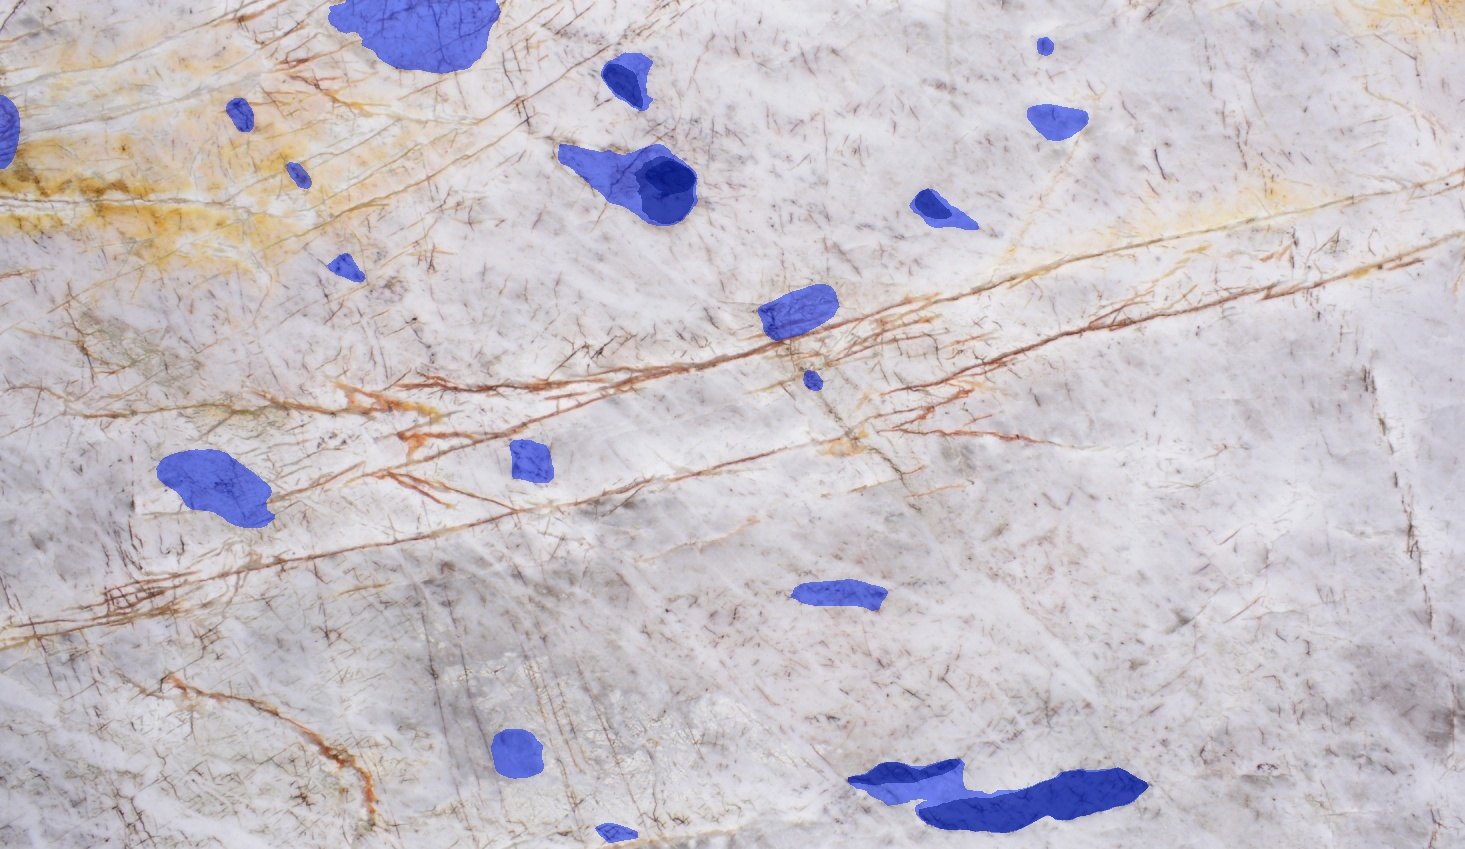
\includegraphics[width=0.45\textwidth]{figuras/sample_ice_leke_darkpatches.jpg}}
  \caption{Decomposição das anotações do SAM por tipo de anomalia na rocha
    \textit{ice leke}. Fonte: elaborado pelo autor.}
  \label{fig:resultado_decomposto}
\end{figure}

\subsection{Análise Preliminar}

Os resultados confirmam a viabilidade da etapa central da proposta: o modelo de fundação, sem treinamento dedicado ao domínio, é capaz de segmentar anomalias relevantes quando guiado por \textit{prompts} calibrados por litologia. As máscaras resultantes são exportadas como polígonos no formato de segmentação do YOLO (coordenadas normalizadas), constituindo o conjunto de \textit{pseudo-labels} que alimentará o treinamento do Aluno. Trata-se de uma validação \textbf{qualitativa e preliminar}: das 45 litologias do conjunto de dados, a \textit{ice leke} é a primeira plenamente calibrada, e a calibração das demais segue em andamento. As métricas quantitativas (mAP e IoU) serão obtidas após o treinamento do Aluno, em etapa posterior.

\section{Considerações Parciais e Trabalhos Futuros}
\label{sec:conclusao}

Este artigo apresentou o ARIA, um \textit{pipeline} hierárquico \textit{Teacher-Student} para a detecção automatizada de anomalias em rochas ornamentais, e suas evidências iniciais. O estágio de classificação está validado (DeepStoneAI) e os resultados sobre a litologia \textit{ice leke} sustentam a viabilidade do uso do SAM como Professor para a geração de anotações por \textit{prompting} calibrado, sem anotação manual extensiva.

As principais limitações desta versão são deliberadas e registradas como trabalhos futuros: o \textbf{loop de aprendizado ativo} (o SAM refinando predições de baixa confiança do YOLO em produção); a \textbf{rotulagem multiclasse} por tipo de anomalia, que requer validação humana de uma amostra das anotações; e a \textbf{integração} do ARIA como serviço da plataforma Hartheus. Os próximos passos imediatos são concluir a calibração das 45 litologias, treinar os modelos especialistas e o \textit{baseline} generalista e realizar a comparação quantitativa que testa a hipótese central.

\bibliographystyle{sbc}
\bibliography{referencias}

\end{document}
